\documentclass[11pt]{article}
\usepackage{etex}
\usepackage{amssymb,amsmath,fancyhdr,multicol}

\usepackage{hyperref}

\usepackage[metapost]{mfpic}

%\pgfplotsset{compat=1.9}
%\usepackage{amsmath}
\usepackage[pdftex]{graphicx}
%\usepackage{mystylefortest}
%\usepackage{multicol}
\usepackage{pst-plot}
\usepackage{pgfplots}

\usepackage{tikz}
\usepackage{tkz-2d}
\usepackage{tkz-base}
\usetikzlibrary{calc}

\usepackage[inline]{enumitem}

\textheight 25cm% 25.5cm
\textwidth 18cm \topmargin -2.5cm
\parindent 0pt
\oddsidemargin -1cm \columnsep 18pt 
\renewcommand{\headrulewidth}{0pt}
\pagestyle{fancy} \lhead{}\chead{}\rhead{}
\lfoot{}\cfoot{}\rfoot{}
%\newcommand{\ds}{\displaystyle}

\usepackage{tabularx}
\renewcommand{\tabularxcolumn}[1]{>{\centering\arraybackslash}m{#1}}

\usepackage{array}
\newcolumntype{?}{!{\vrule width 1pt}}

\usepackage[linewidth=1pt]{mdframed}

%\prec 
\pgfplotsset{compat=1.9} %%May have to change to 1.11 at work

\pgfplotsset{soldot/.style={color=blue,only marks,mark=*}} \pgfplotsset{holdot/.style={color=blue,fill=white,only marks,mark=*}}
\pgfplotsset{
  grid style = {
    dash pattern = on 0.05mm off 1mm,
    line cap = round,
    black,
    line width = 0.5pt
  }
}

\newcommand{\vasymptote}[2][]{
    \draw [densely dashed,thick, #1] ({rel axis cs:0,0} -| {axis cs:#2,0}) -- ({rel axis cs:0,1} -| {axis cs:#2,0});
}

\opengraphsfile{RationalFunctionQuestions}

\begin{document}

\centerline{\textbf{Rational Functions Questions}}

\vspace{.5in}

%\textbf{Name:}\hrulefill\

%\vspace{.25in}

%\makebox[\textwidth]{Name:\enspace\hrulefill}
%\vspace{1pt}

%\begin{questions}


%\addpoints
%\qformat{Question \thequestion\dotfill
 %        {(\pointsofquestion{\arabic{question}} \points)}}
        
\begin{enumerate} 

\item The graph of the rational function $\displaystyle y=\frac{f(x)}{g(x)}$ is shown below.

\begin{minipage}[t]{0.49\linewidth}
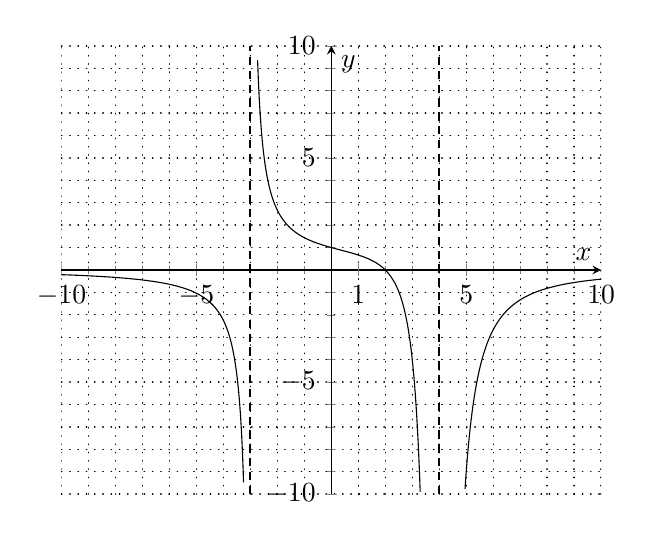
\begin{tikzpicture}
    \begin{axis}[
        restrict y to domain=-10:10,
        samples=1000,
        minor tick num=4,
        xmin = -10, xmax = 10,
        ymin = -10, ymax = 10,
        unbounded coords=jump,
        axis x line=middle,
        axis y line=middle, grid=both,
        extra x ticks={1},
        %extra x tick style={grid=major,
        %tick label style={
        %rotate=90,anchor=east}},
        extra x tick labels={1},
        xlabel=$x$,ylabel=$y$]

      \addplot[mark=none, domain=-10:10] {(48-24*x)/(x^3-5*x^2-8*x+48)};
      \vasymptote {-3}
      \vasymptote {4}
    \end{axis}
  \end{tikzpicture}
  \end{minipage}
\hfill \vrule \hfill
\begin{minipage}[b]{0.5\linewidth}

\begin{enumerate}
\item Write the equations of the vertical asymptotes.


\item Write the equations of the horizontal asymptote.


\item Which of the following best represents the denominator $g(x)$ of the rational function?

\begin{enumerate}
\item $\displaystyle (x+3)(x-4)$
\item $\displaystyle (x+3)^2(x-4)$
\item $\displaystyle (x+3)(x-4)^2$
\item $\displaystyle (x+3)^2(x-4)^2$
\item None of the above
\end{enumerate}

\end{enumerate}
\end{minipage}


\item Assume that a car  has a fuel efficiency of $x$ MPG (miles per gallon), and is driven an average of 10000 miles in one year.

\begin{enumerate}
\item Write a formula for the gas consumption $y$ (in gallons), in terms of $x$.
\item A person plans to trade in her 2009 Honda Civic, which gets 24 MPG, with a 2015 Honda CRX, which gets 28 MPG. How many gallons of gas does she save in one year, assuming that she drives an average of 10000 miles?
\item Another person plans to trade in her 2010 Land Rover Sport, which gets 14 MPG, with a 2015 Land Rover Sport, which gets 16 MPG. How many gallons of gas does she save in one year, assuming that she drives an average of 10000 miles?
\end{enumerate}

\item This problem is from \url{http://tinyurl.com/ratioapp}). 
This application is a Cost-Benefit Model.  A utility company burns coal to generate electricity.  The cost C (in dollars) of removing $x$ amount (percent) of the smokestack pollutants is given by: $\displaystyle C(x)=\frac{80000x}{100-x}$.
\begin{enumerate}
\item Is it possible for the company to remove 100 percent of the pollutants?  
\item What happens if the company does try to remove 100 percent of the pollutants?  Will the company be successful at doing so, or will the attempt end in failure, that is, will it be to much expense for the company?  
\item Find the domain of $C(x)$, based on the physical constraints of the problem.
\end{enumerate}

\end{enumerate}
\end{document}